
\section{Introduction}
\begin{frame}[c]
  \frametitle{Motivation}
     \begin{figure}[h!]
         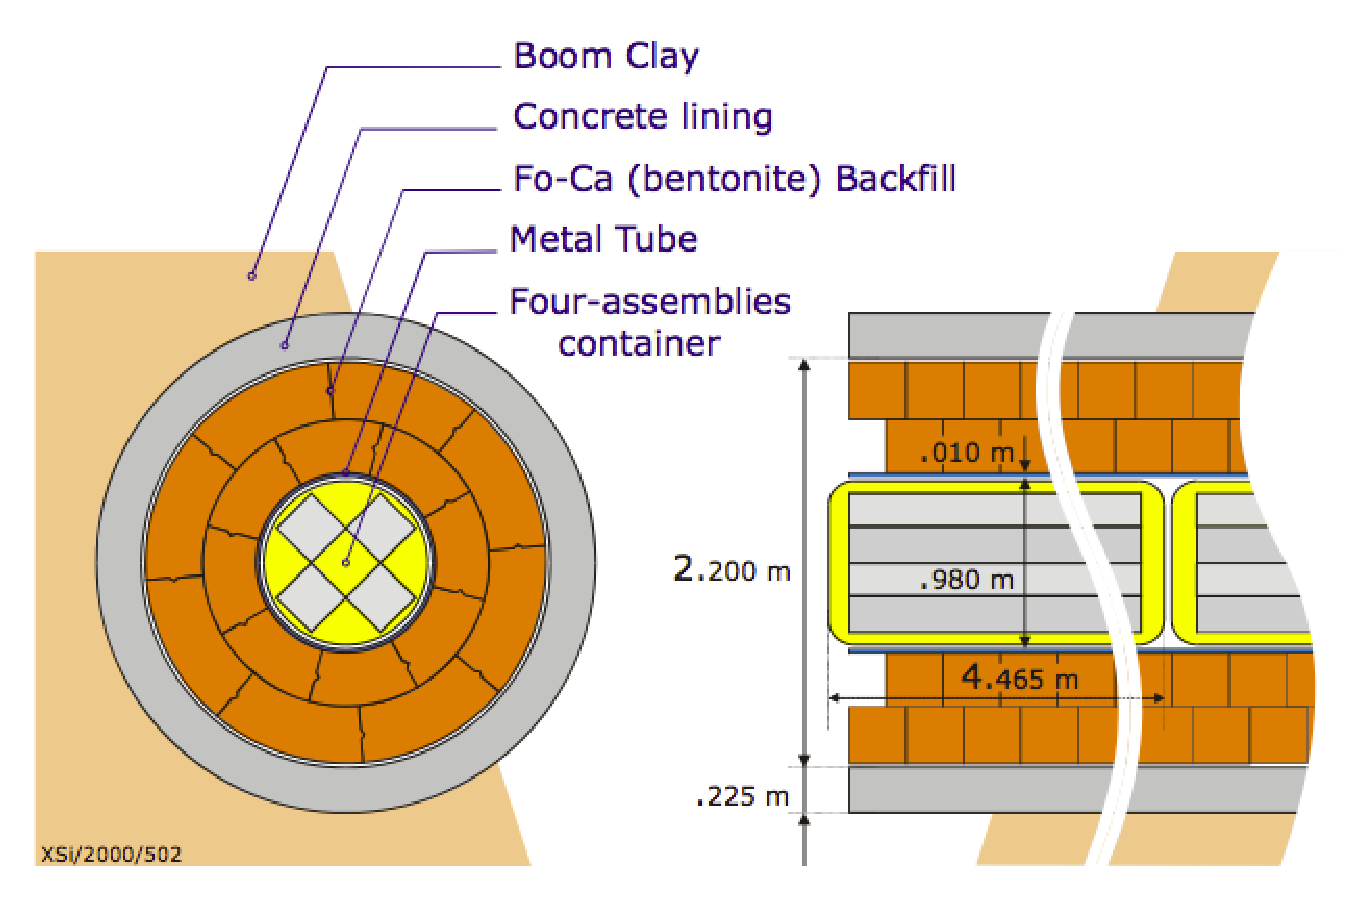
\includegraphics[width=.4\textwidth]{belgianClayRedImp.eps}
         \caption{Belgian reference concept in Boom Clay 
         \cite{von_lensa_red-impact_2008}.}
     \end{figure}
     \begin{figure}[h!]
         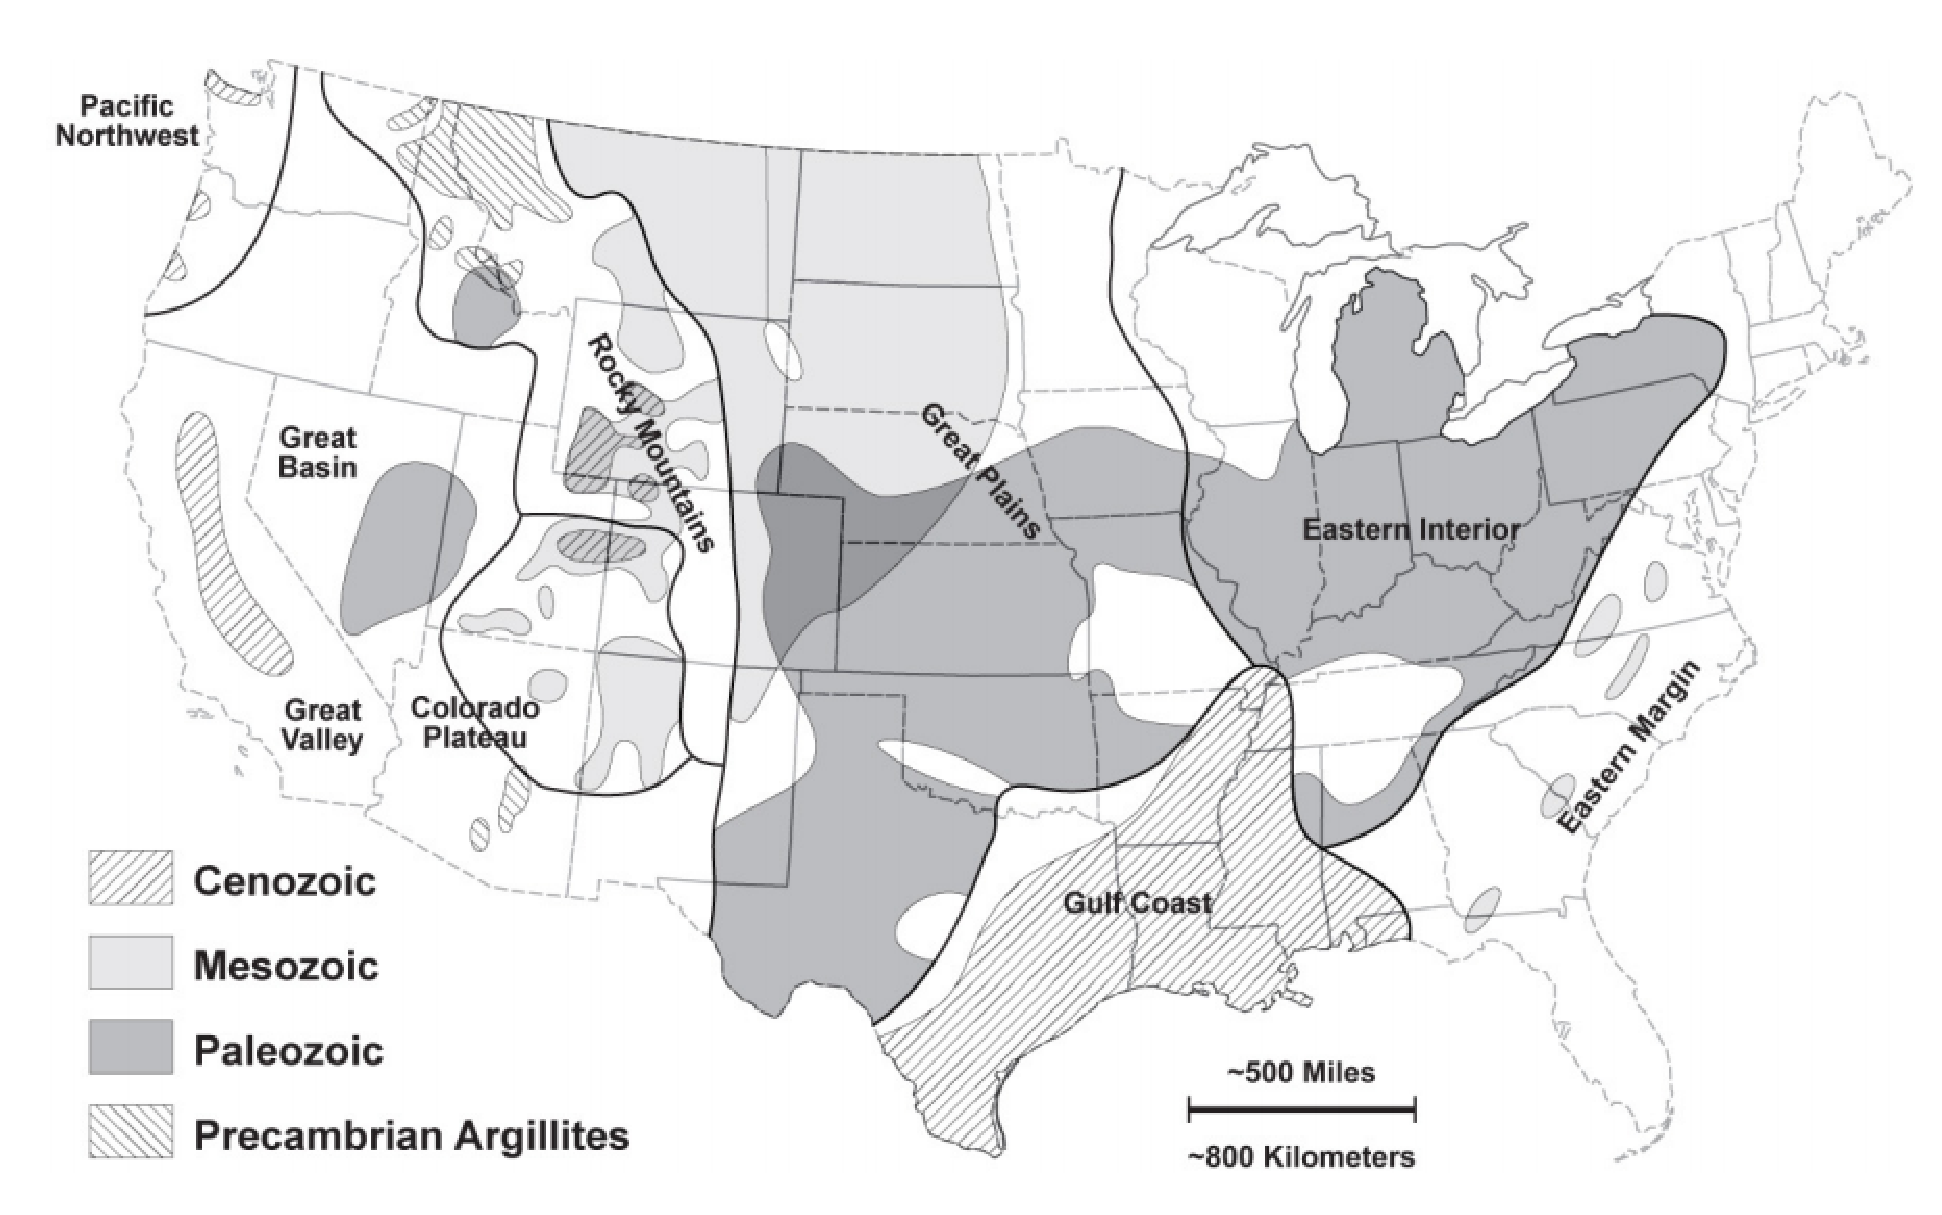
\includegraphics[width=0.4\textwidth]{clayGonzales.eps}
         \caption{U.S. Clay Deposits, ref. \cite{gonzales_shales_1985}.}
     \end{figure}
   \hspace{0.01cm}
\end{frame}

\begin{frame}[c]
  \frametitle{Clay Generic Disposal System Model}
Sensitivity analysis based on the detailed computational \textbf{Clay 
  \gls{GDSE}} developed by the \gls{UFD} campaign \cite{clayton_generic_2011}.  
  was performed with respect to various \textbf{key processes and parameters} 
  affecting long-term post-closure performance of geologic repositories in 
  \textbf{clay} media.

\end{frame}


\begin{frame}[c]
  \frametitle{Clay Generic Disposal System Model}
The Clay \gls{GDSM}, developed at Argonne National Lab, is built on the GoldSim 
simulation framework and contaminant transport model.  It simulates chemical and 
physical attenuation processes \cite{golder_goldsim_2010, 
golder_goldsim_ct_2010}, including 
\begin{itemize}
  \item  chemical and physical attenuation processes including
  \item radionuclide solubility,
  \item dispersion phenomena,
  \item and reversible sorption.
\end{itemize}

Input parameters include 
\begin{itemize}
  \item geometry specifications (e.g. repository depth),
  \item geologic material properties (e.g. clay porosity), 
  \item geochemical data (e.g. elemental solubility limits),
  \item and environmental parameters (e.g. natural system velocity). 
\end{itemize}
\end{frame}

\begin{frame}[c]
  \frametitle{Clay Generic Disposal System Model}
  \vspace{2cm}
\begin{figure}[h!]
\includegraphics[width=0.6\textwidth]{feps.eps}
\caption{General Features Events and Processes in the Clay repository model 
  \ref{clayton_generic_2011}.}
\end{figure}
\end{frame}

\begin{frame}[c]
  \frametitle{Clay Generic Disposal System Model}
The disposal concept modeled by the Clay \gls{GDSM} \cite{nutt_generic_2009} is
\begin{itemize}
  \item an array of spent nuclear fuel packages 
  \item emplaced horizontally
  \item in excavated tunnels, 
  \item backfilled by a reducing bentonite clay,
  \item within a clay repository envrionment, 
  \item \textbf{500 meters} beneath the earth's surface.
\end{itemize}
\end{frame}

\begin{frame}[c]
  \frametitle{Mean of the Peak Annual Dose}
In this analysis, repository performance is quantified by radiation dose to a 
hypothetical receptor. Specifically, the mean of the peak annual dose,

\footnotesize{
  \begin{align} \label{MoP}
    D_{MoP,i} &= \frac{\sum_{r=1}^{N}{\max\left[\left.D_{r,i}(t)\right|_{\forall t}\right]}}{N}
    \intertext{where}
    D_{MoP,i} &= \mbox{ mean of peak annual dose due to isotope i } [mrem/yr]\nonumber\\
    D_{r,i}(t) &= \mbox{ year t dose in realization r due to isotope i } [mrem/yr]\nonumber\\
    N &= \mbox{number of realizations, } \nonumber
\end{align}
}

is a conservative metric of repository performance and should not be confused 
with the peak of the mean annual dose.

\footnotesize{
  \begin{align} \label{PoM}
    D_{PoM,i} &= \max\left[{\frac{\sum_{r=1}^{N}{\left.D_{r,i}(t)\right|_{\forall t}}}{N}}\right]\\
              &= \mbox{peak of the mean annual dose due to isotope i } [mrem/yr].\nonumber
  \end{align}
}
\end{frame}

\begin{frame}[c]
  \frametitle{Sampling Strategy}
  \footnotesize{
To develop a many dimensional overview, both individual and dual parametric cases were performed.

\begin{itemize}
  \item \textbf{Individual parameter cases} varied a single parameter of interest in 
detail over a broad range of values. 
  \item \textbf{Dual parameter cases} were performed for pairs of parameters expected to exhibit some covariance. 
\end{itemize}    
For each case, forty simulation 
groups varied the parameter or parameters within the range considered. 
For each simulation group, a 100 realization simulation was completed 
\cite{clayton_generic_2011, 
nutt_generic_2009}.  

\begin{table}[ht!]
\centering
\footnotesize{
\begin{tabular}{|l|l|l|r|r|}
\multicolumn{5}{c}{\textbf{Simulation Cases}}\\
\hline
\textbf{Case} & \textbf{Parameter} & \textbf{Units} & \textbf{Min. Value} & \textbf{Max. Value}\\
\hline
V     & $R_{WFDeg.}$           & $[yr^{-1}]$       & $10^{-9}$    &  $10^{-2}$ \\
      & Inventory              & [MTHM]         & $10^{-4}$    &  $10^1$ \\
\hline
\end{tabular}
\caption{Each dual and single parameter simulation case had 40 simulation 
groups of 100 realizations each.}
\label{tab:Cases}
}
\end{table}


}

\end{frame}
